\documentclass[10pt]{article}
\usepackage[margin=17mm]{geometry}
\usepackage{graphicx,booktabs,hyperref}
\usepackage[strings]{underscore}
\setlength{\parindent}{0pt}\setlength{\parskip}{4pt}
\begin{document}
\section*{Independent native pricing reconstruction}
Post-outcome accounting audit, 2026-10-25, source frozen at db732b62b.
This explicitly corrects the earlier n=13/n=23 solver-wall-pricing description.
The native auditor reconstructs every available IC charge from integer
counts and fixed prices, checking the raw total and the solver component.
It also checks the ordinary band wherever that band is available.

The completed n=13 and n=23 structured solvers use pinned word rates,
0.002304 and 0.001164 GAE per word. The n=7 measured solver term is removed
by ic_report. Elapsed solver time is a diagnostic and contributes no wall
charge to these reported costs. Raw S remains incomplete: symbolic
construction and splitting are not fully counted. Original PDFs and
sealed data are preserved; corrected n13/n23 reports supersede their pricing
paragraph. Missing cost does not become zero through this correction.

\begin{center}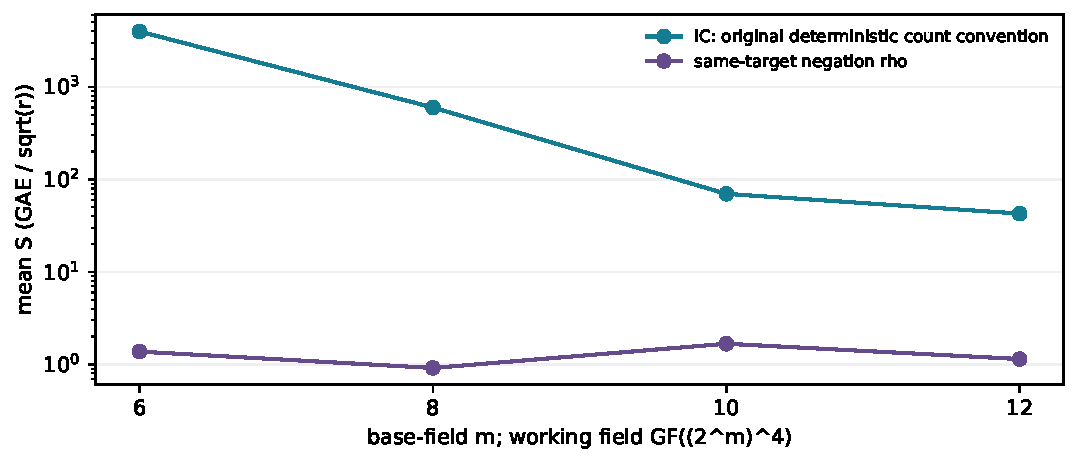
\includegraphics[width=.98\linewidth]{quartic-recorded-costs.pdf}\end{center}
\begin{center}\begin{tabular}{rrr}\toprule
Base m & original IC S, mean of 2 & negation rho S, mean of 2\\\midrule
6 & 3978.13 & 1.37576 \\
8 & 599.899 & 0.91547 \\
10 & 69.8954 & 1.67309 \\
12 & 42.7541 & 1.14273 \\
\bottomrule\end{tabular}\end{center}

The quartic raw convention counts Fq solver operations and converts them
using a deterministic operations-per-addition ratio. Successful-lift prices
are reconstructed from 32 probes with seed 0x5e. Public constructor inputs,
order, subgroup and generator coordinates are independently checked against
each raw record. The virtual ratios are count conventions, not measured
nanoseconds or hardware calibration. Both rho repeats retain exactly equal
deterministic counts. These are two known-answer one-target workloads per
rung at L0; no population interval or physical crossover is established.
Scalar replay of the smoke is separate from this accounting audit.

\newpage
\section*{Quartic band scope and retained refusal}
The current canonical ecbench band refuses these constructed curves because
their adapter-created virtual calibration rows were not persisted in the
global table. The exact command, output and status are retained beside this
audit. No global hardware calibration or sealed record is rewritten.

\begin{center}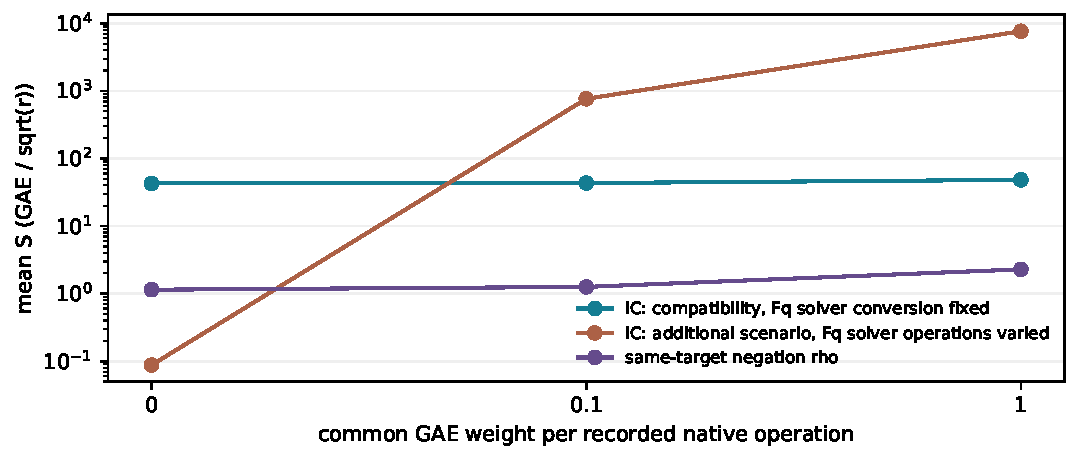
\includegraphics[width=.98\linewidth]{quartic-accounting-scenarios.pdf}\end{center}

At m=12, compatibility means at weights 0/0.1/1 are 42.72275 / 43.27648 / 48.26008.
This reconstructs the existing band's arithmetic and holds the counted Fq
solver conversion fixed, as that implementation does. The additional
all-native scenario also varies those Fq solver operations; its means are
0.08756439 / 763.8111 / 7637.323. This is a separately labeled accounting scenario, not an
algorithm change, a speedup or a redefinition of old S. All means require
every planned target to verify; censored or failed arms have null means.

The complete-price obligation remains open for construction, splitting,
word scans and physical conversion. The graph at weight zero must not be
used to claim an IC win. No result is promoted to the performance leaderboard
or admitted benchmark table. The separate structural scoreboard panel changes
only its incorrect pricing description; historical performance plots are
unchanged because this audit adds no algorithmic improvement.

Raw evidence: \path{../../pipeline-receipts/pricing-audit-20261025/receipt.json}.
Protocol: \path{../../PRICING_AUDIT_PROTOCOL.md}.
Native source: \path{examples/ic_campaign_pricing_audit.rs}.
Reproduction command and byte-comparison record, source/input/binary hashes,
limits and exit status are beside the receipt. Sealed input sessions:
\path{../../pipeline-runs/structured-n7-20261025-01/}, n13, n23,
and \path{../../pipeline-runs/quartic-smoke-20261025-02/}.

\end{document}
